\section{Zahlendarstellung}
\label{sec:zahlendarstellung}

\textbf{Zahlensysteme -- Stellenwertsystem}
\begin{items}
	\item Darstellung einer Zahl durch Ziffern $z_i$ -- Stellenwert $i$te Position: $i$te Potenz der Basis $b$
	\item Wert $X_b = \sum _{i=-m}^n z_ib^i$
	\item Wichtige Zahlensysteme: Dual-, Oktal-, Dezimal-, Hexadezimalsystem
\end{items}
\begin{figure}[ht]
  \centering
  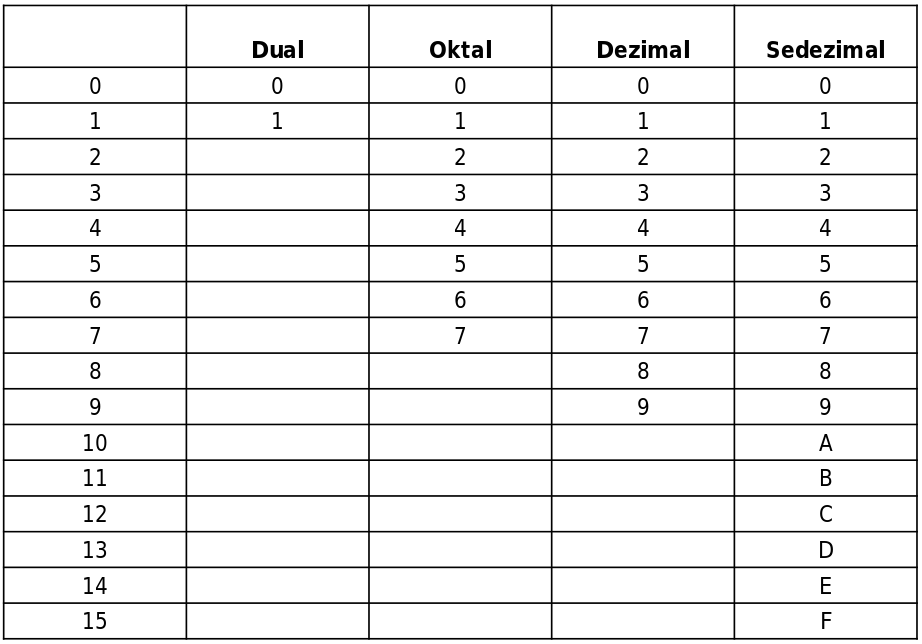
\includegraphics[width=0.33\textwidth]{Zahlensysteme}
  \label{Zahlensysteme}
\end{figure}

\textbf{Umwandlung von Dezimal zu Basis $b$}
\begin{enumeration}
	\item \underline{euklidischer Algorithmus}:
	\begin{enumeration}
		\item Berechne $p$ mit $b^p \leq Z < b^{p+1}$, setze $i=p$
		\item Berechne $y_i=Z_i \text{ div } b^i$, $R_i = Z_i \text{ mod } b^i$
		\item Wiederhole (b)H für $i= p-1,\dots$, ersetze dabei $Z$ durch $R_i$, bis $R_i=0$ oder $b^i$ klein genug ist
	\end{enumeration}
	\begin{align*}
		2^3 \leq \ &13 < 2^4 \\
		13:2^3 &= 1 \text{ Rest } 5 \\
		5:2^2 &= 1 \text{ Rest } 1 \\
		1:2^1 &= 0 \text{ Rest } 1 \\
		1:2^0 &= 1 \text{ Rest } 0 \\
		\leadsto Z=13_{10} &= 1101_2
	\end{align*}

	\item \underline{Horner-Schema}:
	\begin{enumeration}
	 	\item ganzzahliger Teil: $15741_{10}$ in Hexadezimal:
			\begin{align*}
				15741_{10}:16 &= 983 \text{ Rest } 13 \ (=D_{16}) \\
				983_{10}:16 &= 61 \text{ Rest } 7 \ (=7_{16}) \\
				61_{10}:16 &= 3 \text{ Rest } 13 \ (=D_{16}) \\
				3_{10}:16 &= 0 \text{ Rest } 3 \ (=3_{16}) \\
				\leadsto Z=15741_{10} &= 3D7D_{16}
			\end{align*}
		\item Nachkommateil: $0,233_{10}$ in Hexadezimal:
			\begin{align*}
				0,233_{10}*16 &= \underline{3},728 \\
				0,728_{10}*16 &= \underline{11},648 \\
				0,648_{10}*16 &= \underline{10},368 \\
				0,368_{10}*16 &= \underline{5},888 \\
				\leadsto Z=0,233_{10} &\approx 0,3BA5_{16}
			\end{align*}
	 \end{enumeration} 
\end{enumeration}

\textbf{Umwandlung Basis $b$ zu Dezimal}
\begin{items}
	\item Einzelne Stellen nach Stellenwertgleichung addieren
	\begin{multline*}
		101101,1101_2 = \\ 2^{-4}+2^{-2}+2^{-1}+2^0+2^2+2^3+2^5 \\ = 45,8125_{10}
	\end{multline*}
\end{items}

\textbf{Umwandlung Basis $b_1$ zu Basis $b_2$}
\begin{enumeration}
	\item Umwandlung über Dezimalsystem
	\item Ist eine Basis Potenz der anderen, so können mehrere Stellen zu einer Ziffer zusammengefasst werden
	\begin{equation*}
		0110100,110101_2 = 0011 \ 0100,1101 \ 0100 = 34,D4_{16}
	\end{equation*}
\end{enumeration}

\newpage

\textbf{Darstellung negativer Zahlen}
\begin{enumeration}
	\item \underline{Betrag und Vorzeichen}: Erstes Bit von Links ist Vorzeichen, Rest ist Betrag (\code{0001 \ 0010 = 18, 1001 \ 0010 = -18})
	\begin{items}
		\item \textbf{Vorteile}: Symmetrischer Zahlenbereich
		\item \textbf{Nachteile}: Darstellungsänderung bei Bereichserweiterung, gesonderte Vorzeichenbehandlung bei Addition und Subtraktion, doppelte Darstellung der Null
	\end{items}

	\item \underline{Einerkomplement}: Negative Zahl = NOT(positive Zahl)
	\begin{center}
		\code{0000 = 0} \quad \code{1111 = -0} \\*
		\code{0001 = 1} \quad \code{1110 = -1} \\*
		\code{0010 = 2} \quad \code{1101 = -2} \\*
		\code{0011 = 3} \quad \code{1100 = -3} \\*
		...
	\end{center}
	\begin{items}
		\item \textbf{Vorteile}: Symmetrischer Zahlenbereich, keine gesonderte Betrachtung des ersten Bits
		\item \textbf{Nachteile}: doppelte Darstellung der Null
	\end{items}

	\item \underline{Zweierkomplement}: = Einerkomplement + 1
	\begin{center}
		\code{0000 = 0} \quad \code{1111 = -1} \\*
		\code{0001 = 1} \quad \code{1110 = -2} \\*
		\code{0010 = 2} \quad \code{1101 = -3} \\*
		\code{0011 = 3} \quad \code{1100 = -4} \\*
		...
	\end{center}
	\begin{items}
		\item \textbf{Vorteile}: Wie Einerkomplement, eindeutige Null
		\item \textbf{Nachteile}: Asymmetrischer Zahlenbereich (eine negative Zahl mehr)
	\end{items}

	\item \underline{Exzess-Darstellung}: Verschiebung nach oben derart, dass kleinste negative Zahl die Darstellung \code{0...0} hat
\end{enumeration}

\textbf{Darstellung von Kommazahlen}
\begin{enumeration}
	\item \underline{Festkommazahlen}: Komma sitzt an einer festen Stelle

	\item \underline{Gleitkommazahlen}: $X = \pm \text{Mantisse}*b^{\text{Exponent}}$ ($b$ fest)
	\begin{items}
		\item $X = (-1)^{\text{Vorzeichen}}*(0,\text{Mantisse})*b^{\text{Exponent}}$
		\item $\text{Exponent} = \text{Charakteristik}-b^{(y-1)-x}$
	\end{items}
	\begin{figure}[ht]
	  \centering
	  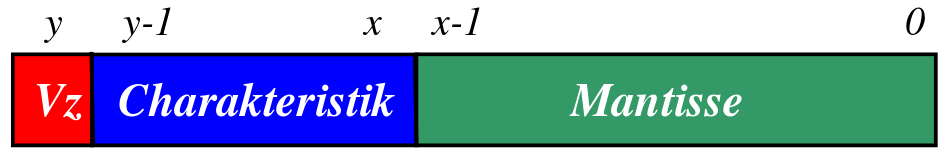
\includegraphics[width=0.33\textwidth]{Gleitkommazahl}
	  \label{Gleitkommazahl}
	\end{figure}

	\item \underline{IEEE-Standard}:
	\begin{enumeration}
		\item 32-Bit:
			\begin{figure}[ht]
			  \centering
			  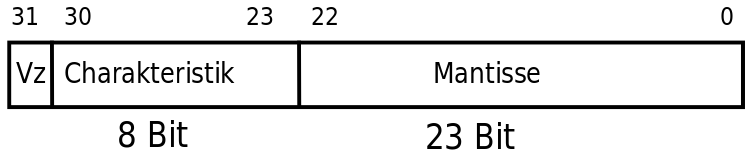
\includegraphics[width=0.33\textwidth]{IEEE-32bit}
			  \label{IEEE-32bit}
			\end{figure}
		\item 64-Bit:
			\begin{figure}[ht]
			  \centering
			  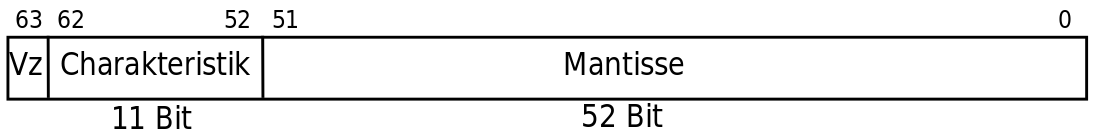
\includegraphics[width=0.33\textwidth]{IEEE-64bit}
			  \label{IEEE-64bit}
			\end{figure}
	\end{enumeration}
\end{enumeration}

\textbf{Codierungen}
\begin{enumeration}
	\item \underline{BCD}: Dezimalzahl ziffernweise als Binärzahl (=\emph{Tetrade}) codieren:
	\begin{center}
		\code{8127 = 1000 \ 0001 \ 0010 \ 0111}
	\end{center}
	\textbf{Nachteil}: Verbraucht viel Speicher, ungeschickt zum Rechnen

	\item \underline{ASCII}: 7-Bit-Codierung zur Textdarstellung

	\item \underline{Unicode}: Weltweit genormte Codierung aller Zeichen (wegen der vielen inkompatiblen ASCII-Derivaten)
\end{enumeration}